%%% Document Author: J Moss
%%% Parts in LaTeX: Nicholas Dart
%%% Other Content: See authors list
%%% Document Last edit: 28.10.2014

\documentclass[11pt, article]{article}
\usepackage{a4wide}
\usepackage[english]{babel}
\usepackage{graphicx}
\usepackage{tabu}
\usepackage{textcomp}
\usepackage{fancyhdr}
\usepackage{lastpage}
\usepackage{titlesec}
\usepackage{lscape}
\usepackage{hyperref}

%%%%%%
%% Variables for version and release status
%% useage: \version
%%%%%%
\newcommand\version{Max Atkins}
\newcommand\release{CS22310 Assignment}
\newcommand\titleText{North Ceredigion Fitness Website Prototype Development}
\newcommand\reference{CS22310 Assignment}

%%%%%%
%% Alias
%%%%%%
\newcommand{\sectionbreak}{\clearpage} 	%% Allways start a section on a new page

\title{ \huge CS22310 - User Centred Design and Human Computer Interaction\\ \Large \titleText}
\author{
	\vspace{100pt}
	\begin{tabular}{ r || l }
		Author 	& Max Atkins \\
						& \\
		Date Published  & \today \\
						&\\
		Department		& Computer Science \\
						&\\
		Address			& Aberystwyth University \\
						& Penglais Campas \\
						& Ceredigion \\
						& SY23 3DB \\
	\end{tabular} \\
	Copyright \textcopyright Aberystwyth University 2015
	%get rid of the date on the titlepage
	\date{}
}

\pagestyle{fancy}
\fancyhf{}
\rhead{\version}
\lhead{\release}
\rfoot{Page \thepage \hspace{1pt} of \pageref{LastPage}}
\lfoot{Aberystwyth University - Computer Science}

\begin{document}
	\setcounter{page}{1}

	\maketitle

	\tableofcontents

	\section{Introduction}
		%%\input{foo/bar.tex}

	\section{Task Analysis}
	
	\subsection{Who is Involved}
	This rich picture diagram highlights who is involved in the website, who can do what, and where data would go. It gives a very broad overview of the entire system.
		\begin{figure}[ht!]
	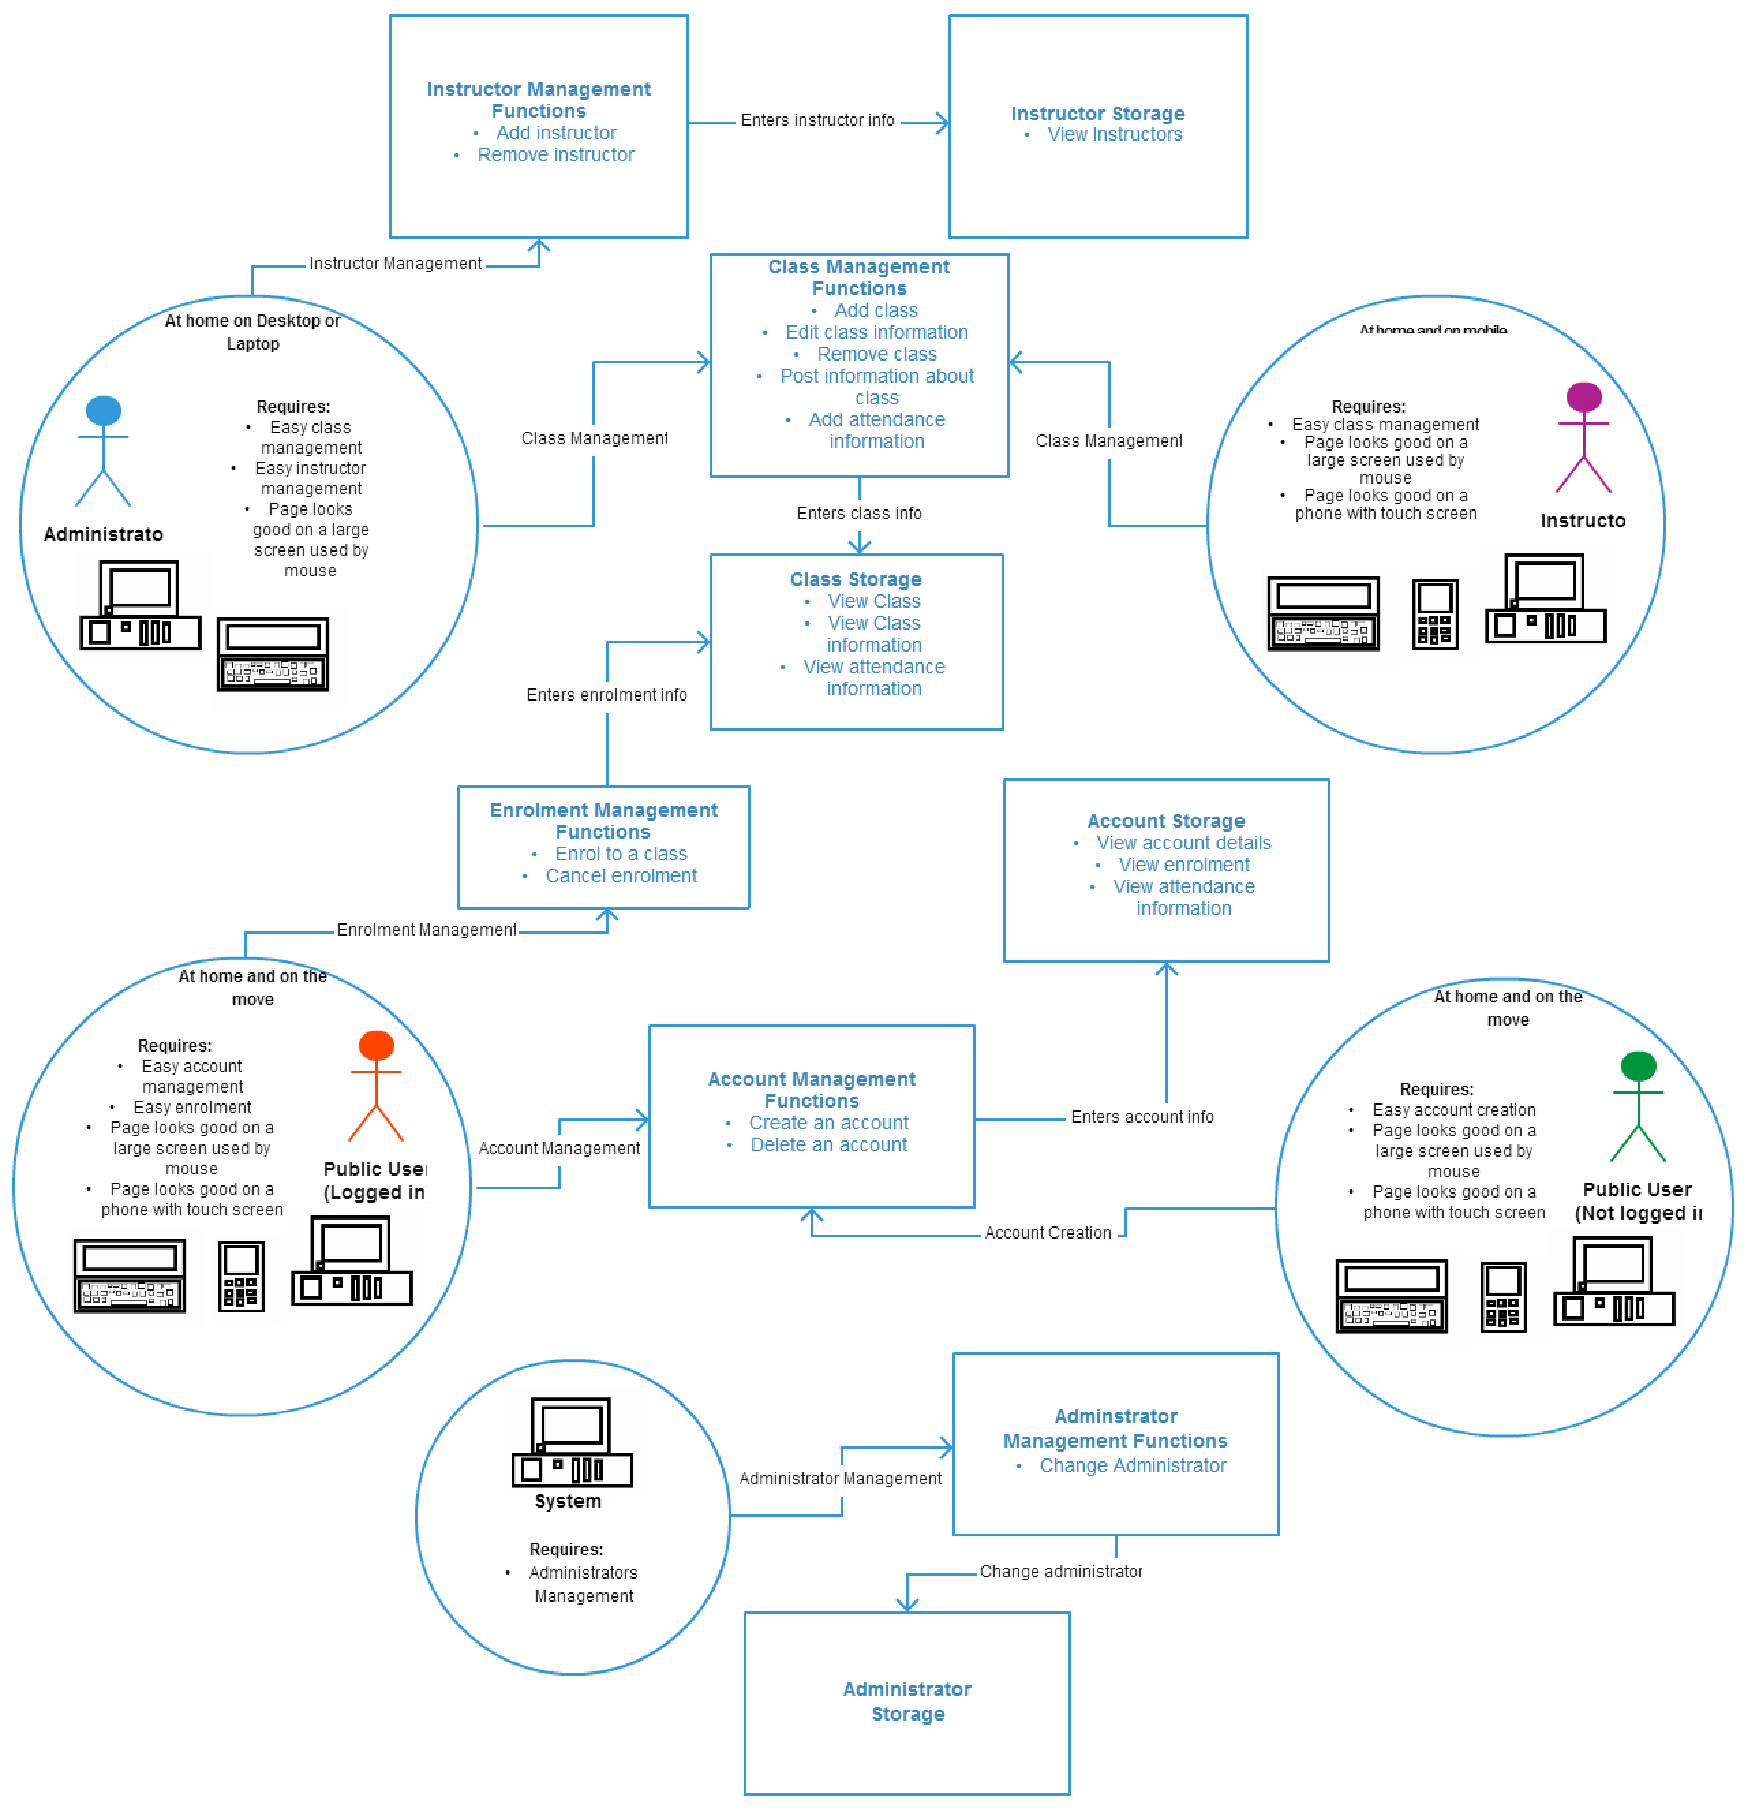
\includegraphics[scale=0.55]{images/richpicture}
 	\caption{Rich Picture}
	\end{figure}
	
	\newpage
	
	\subsection{Tasks the System Performs}
	This use-case diagram details all the functionality required by the website, and who can perform each function.
	\begin{figure}[ht!]
	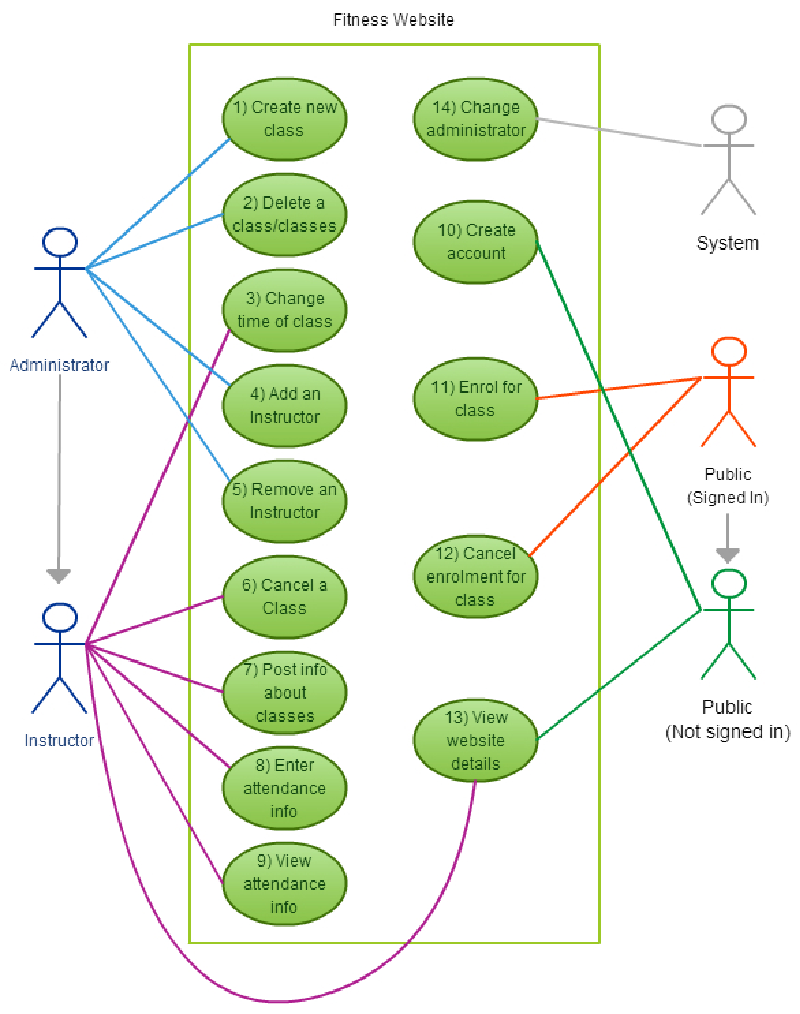
\includegraphics[scale=1]{images/usecase}
 	\caption{Use-Case Diagram}
	\end{figure}
	
	\newpage
	
	\subsection{How Tasks and Data Relate}
	This dataflow diagram is an extension of the use-case, but shows where the data will flow in the system and where the data will be stored.
		\begin{figure}[ht!]
	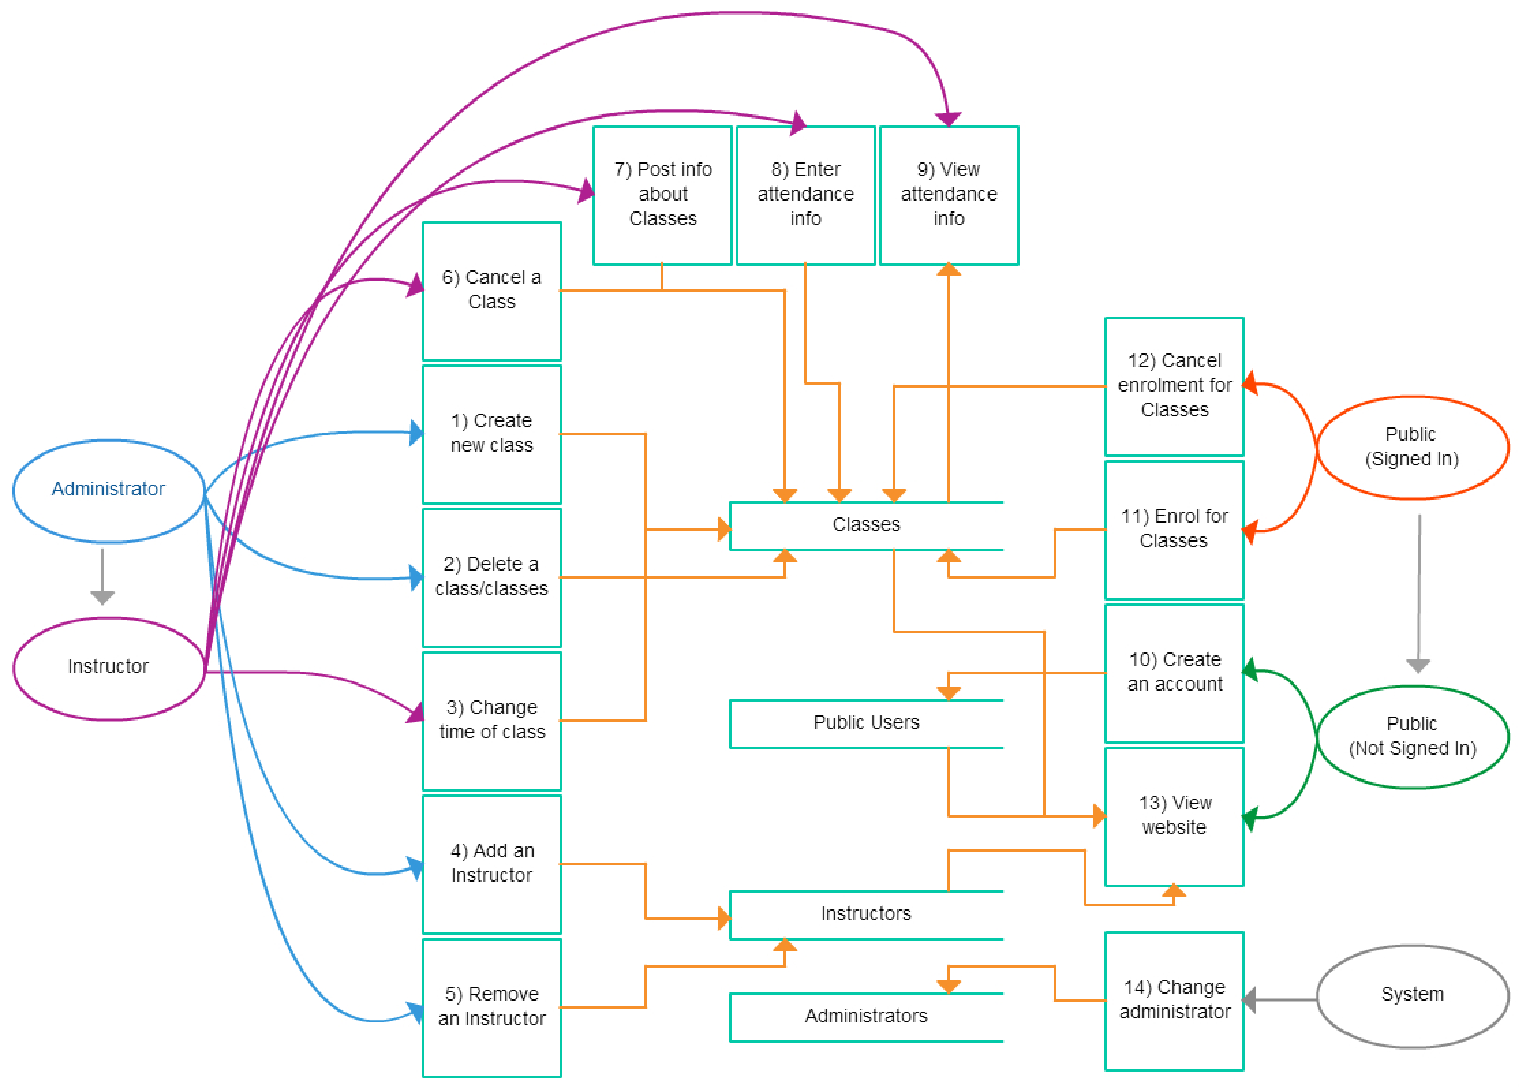
\includegraphics[scale=0.6]{images/dataflow}
 	\caption{Dataflow Diagram}
	\end{figure}
	
	\newpage
	\subsection{How Tasks are Related}
	This state transition diagram shows each possible state of the system. Please note that, to save space and confusion, states are preserved when returning to the Existing Classes state in the middle. 
			\begin{figure}[ht!]
	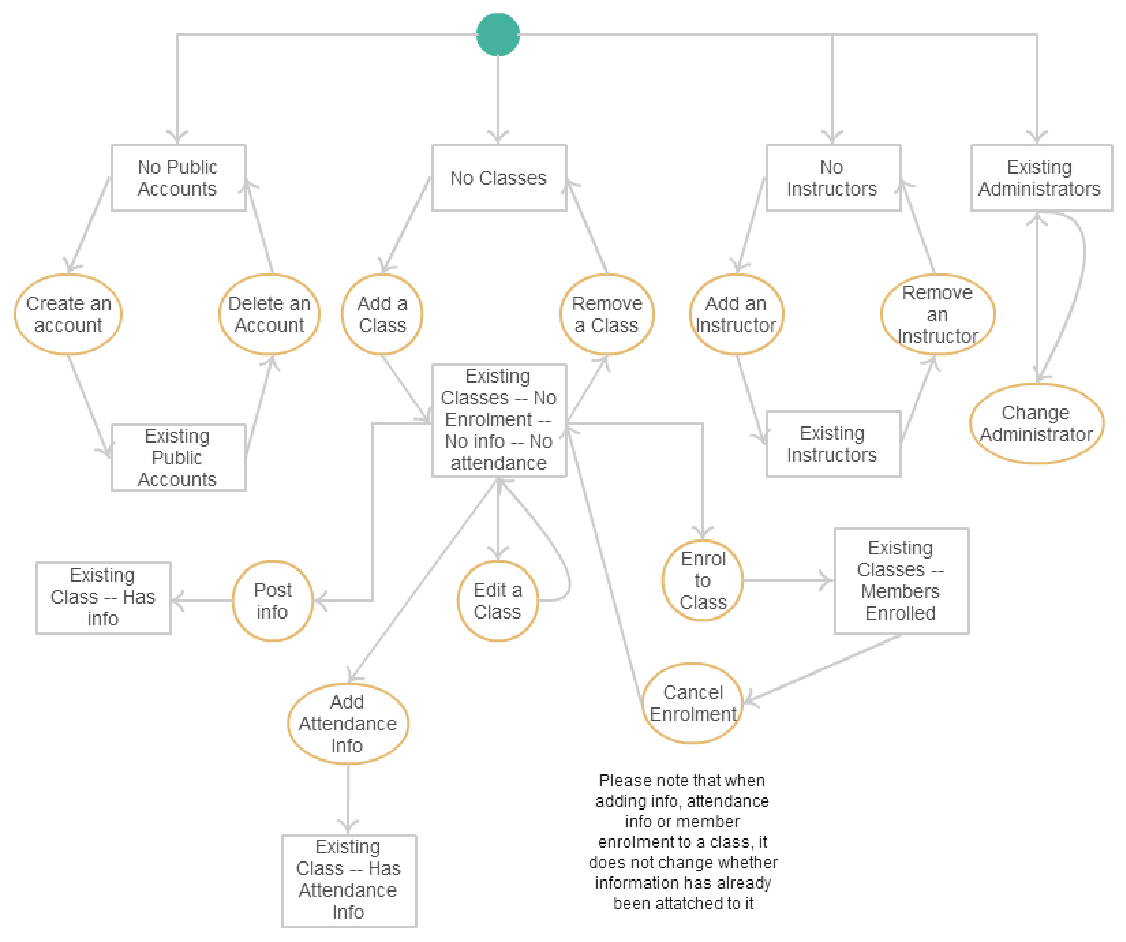
\includegraphics[scale=0.8]{images/statediagram}
 	\caption{State Transition Diagram}
	\end{figure}
	
	\section{High-Level Design}

	\subsection{Sketches of UI}

			\begin{figure}[ht!]
	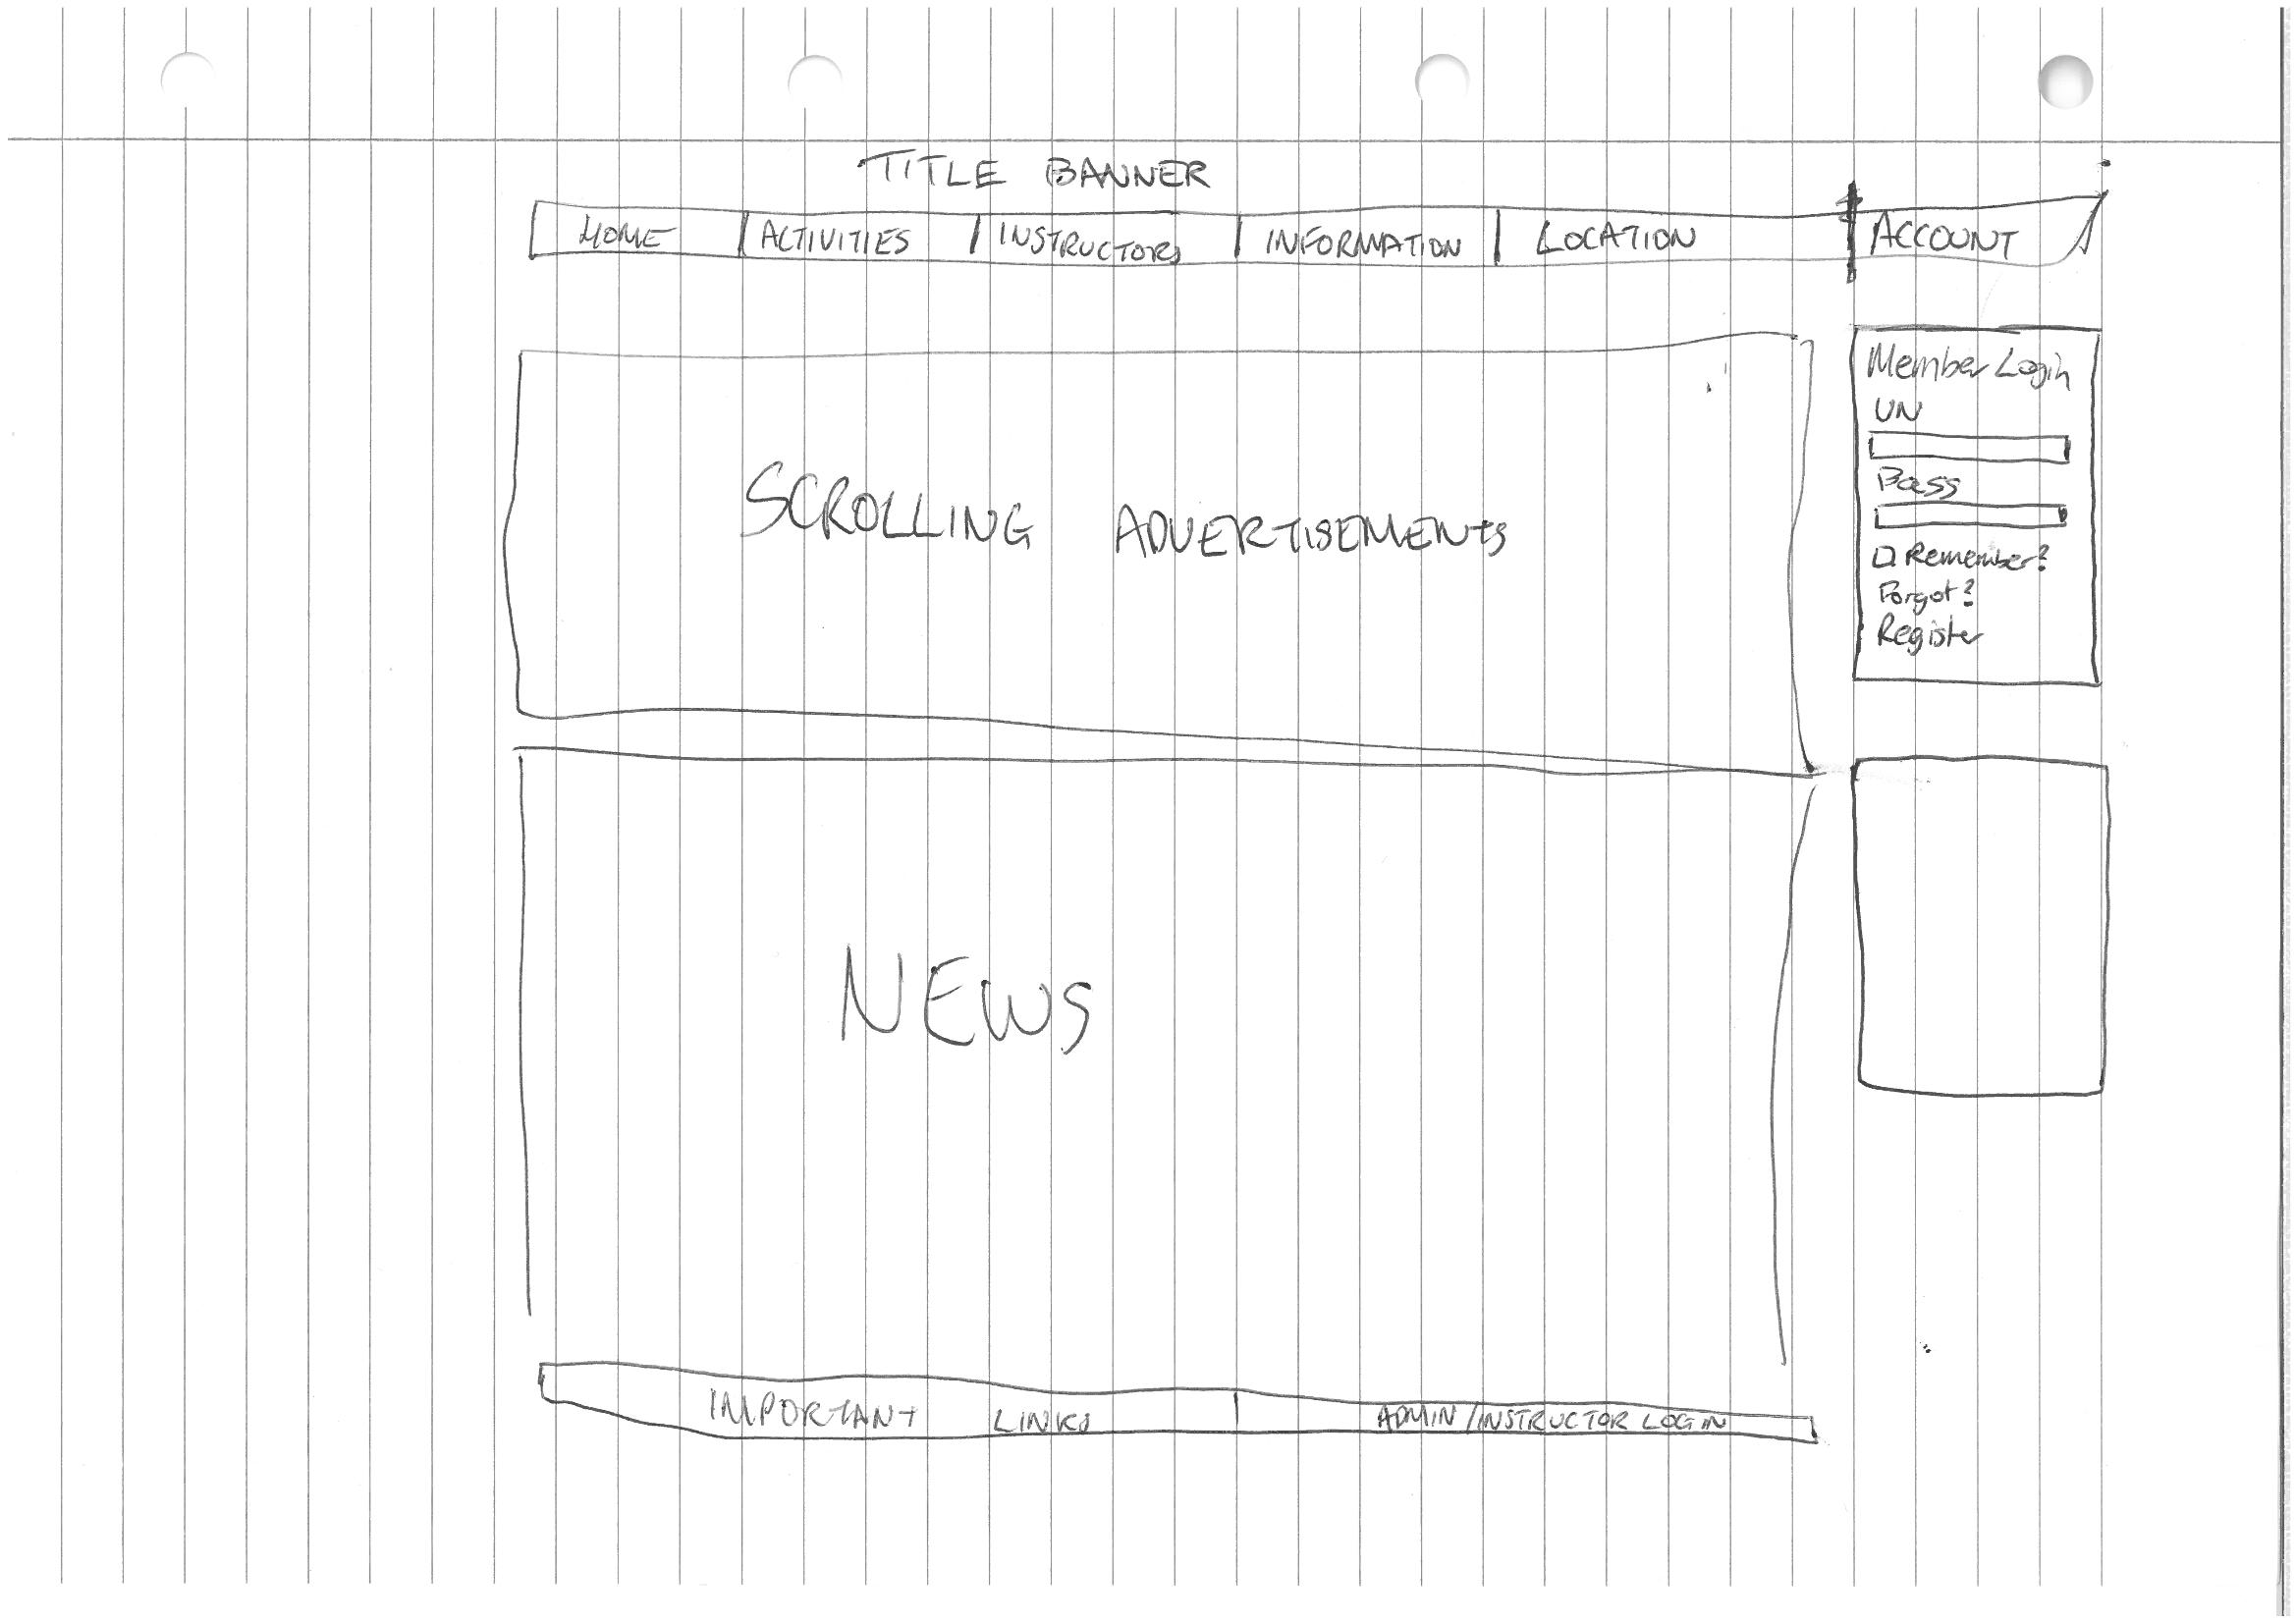
\includegraphics[scale=0.7]{images/homepage}
 	\caption{Homepage}
	\end{figure}
1: A nice and simple navigation bar that will show the user where to go in the site. When hovered over, each button will highlight, achieving Schneiderman's 3rd rule. When changing page, the active page will stay highlighted. This supports Schneiderman's 7th rule.

2: Two windows for textual/image-based content are provided and more can be easily implemented creating a scrollable, interactive homepage.

3: Accessibility options such as increasing the text size and high contrast to achieve Schneiderman's 2nd rule.

4: A member login box that provides login functionality, forgotten password, remember my details and register options.
\newpage
			\begin{figure}[ht!]
	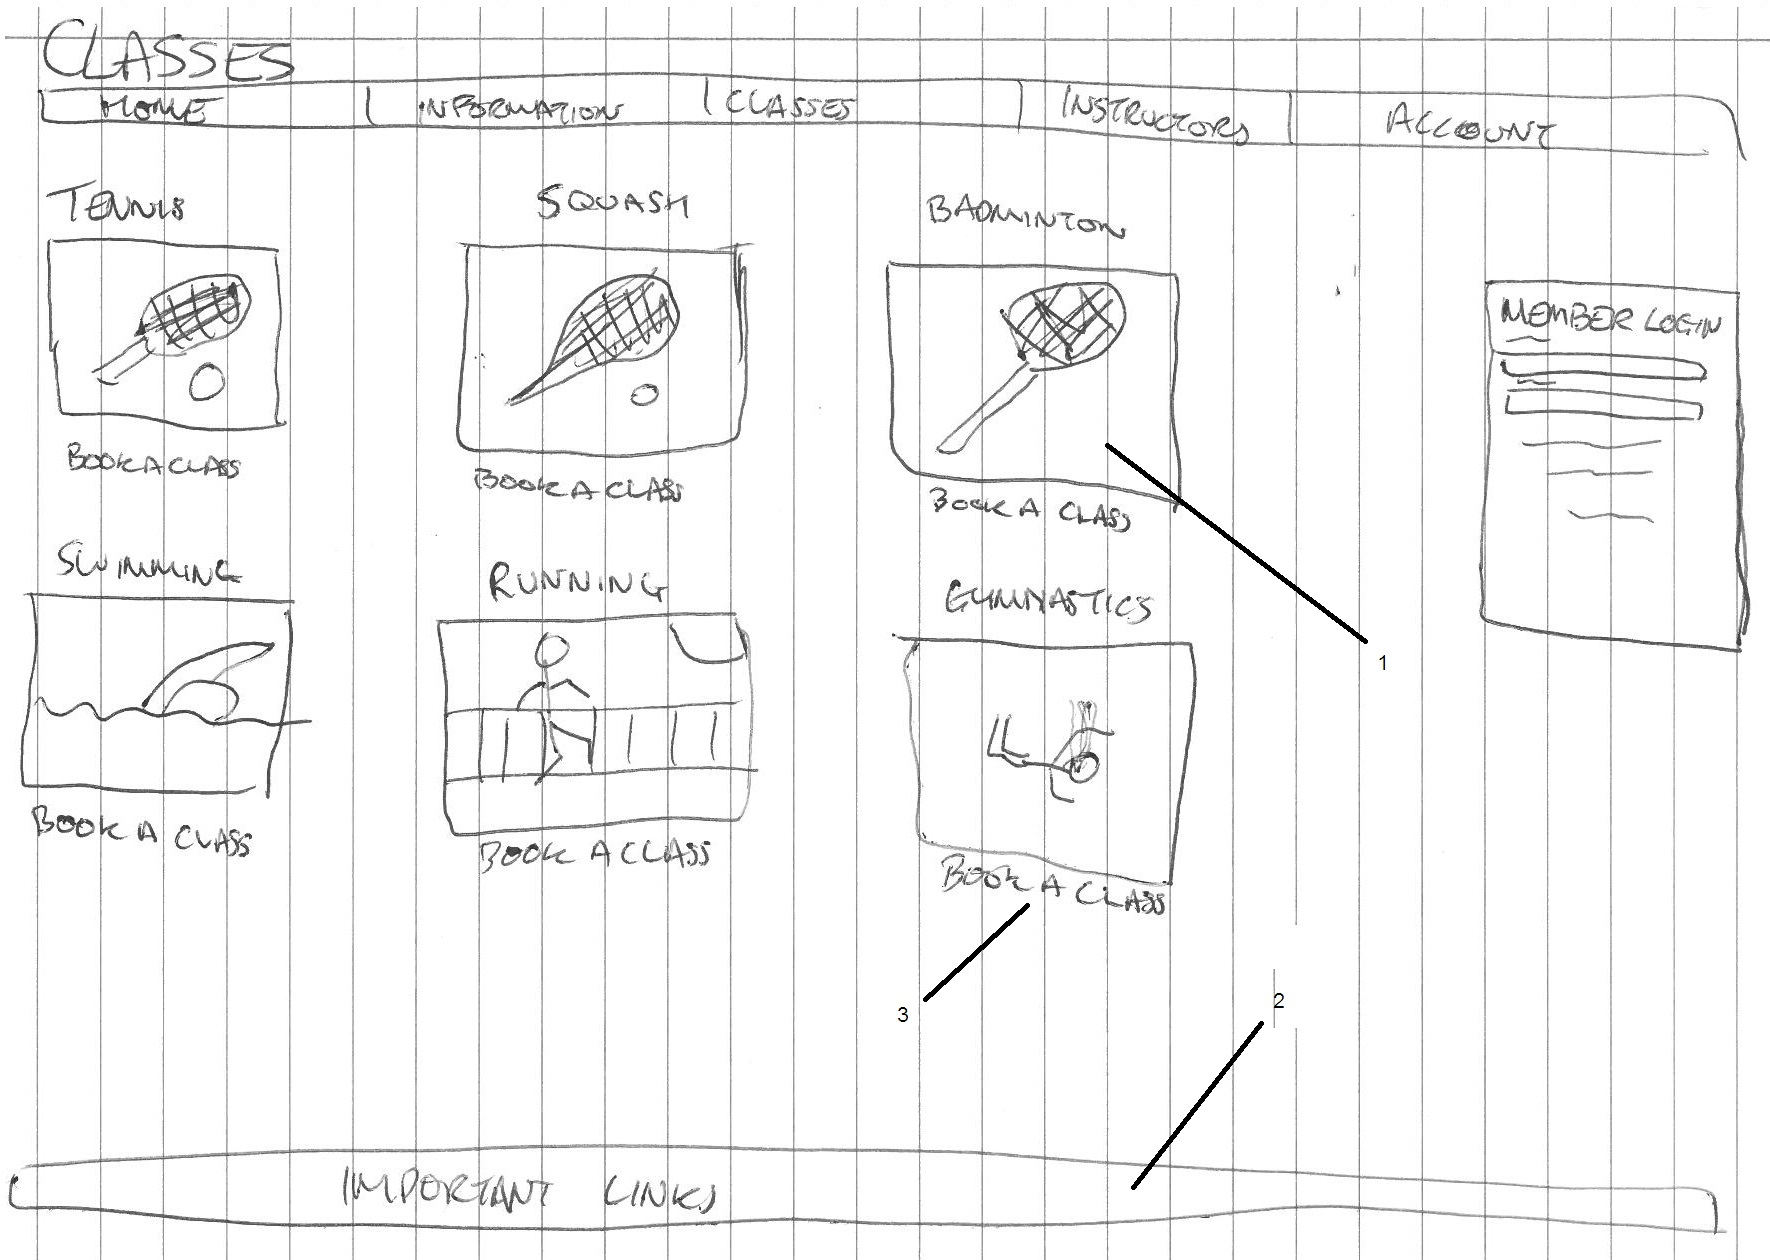
\includegraphics[scale=0.7]{images/classpage}
 	\caption{Class Listings Page}
	\end{figure}	
1: A nice, user-friendly grid system that can be responsive and mobile-friendly. Images are shown to reduce load on user-memory in accordance to Schneiderman's 8th rule.

2: Important links are displayed at the bottom for people wanting to go further into the site. Contains links to legal information, sitemap etc. 

3: Book a class links are displayed to allow the user to easily find what they want. Information about the class will also be displayed here.
\newpage
			\begin{figure}[ht!]
	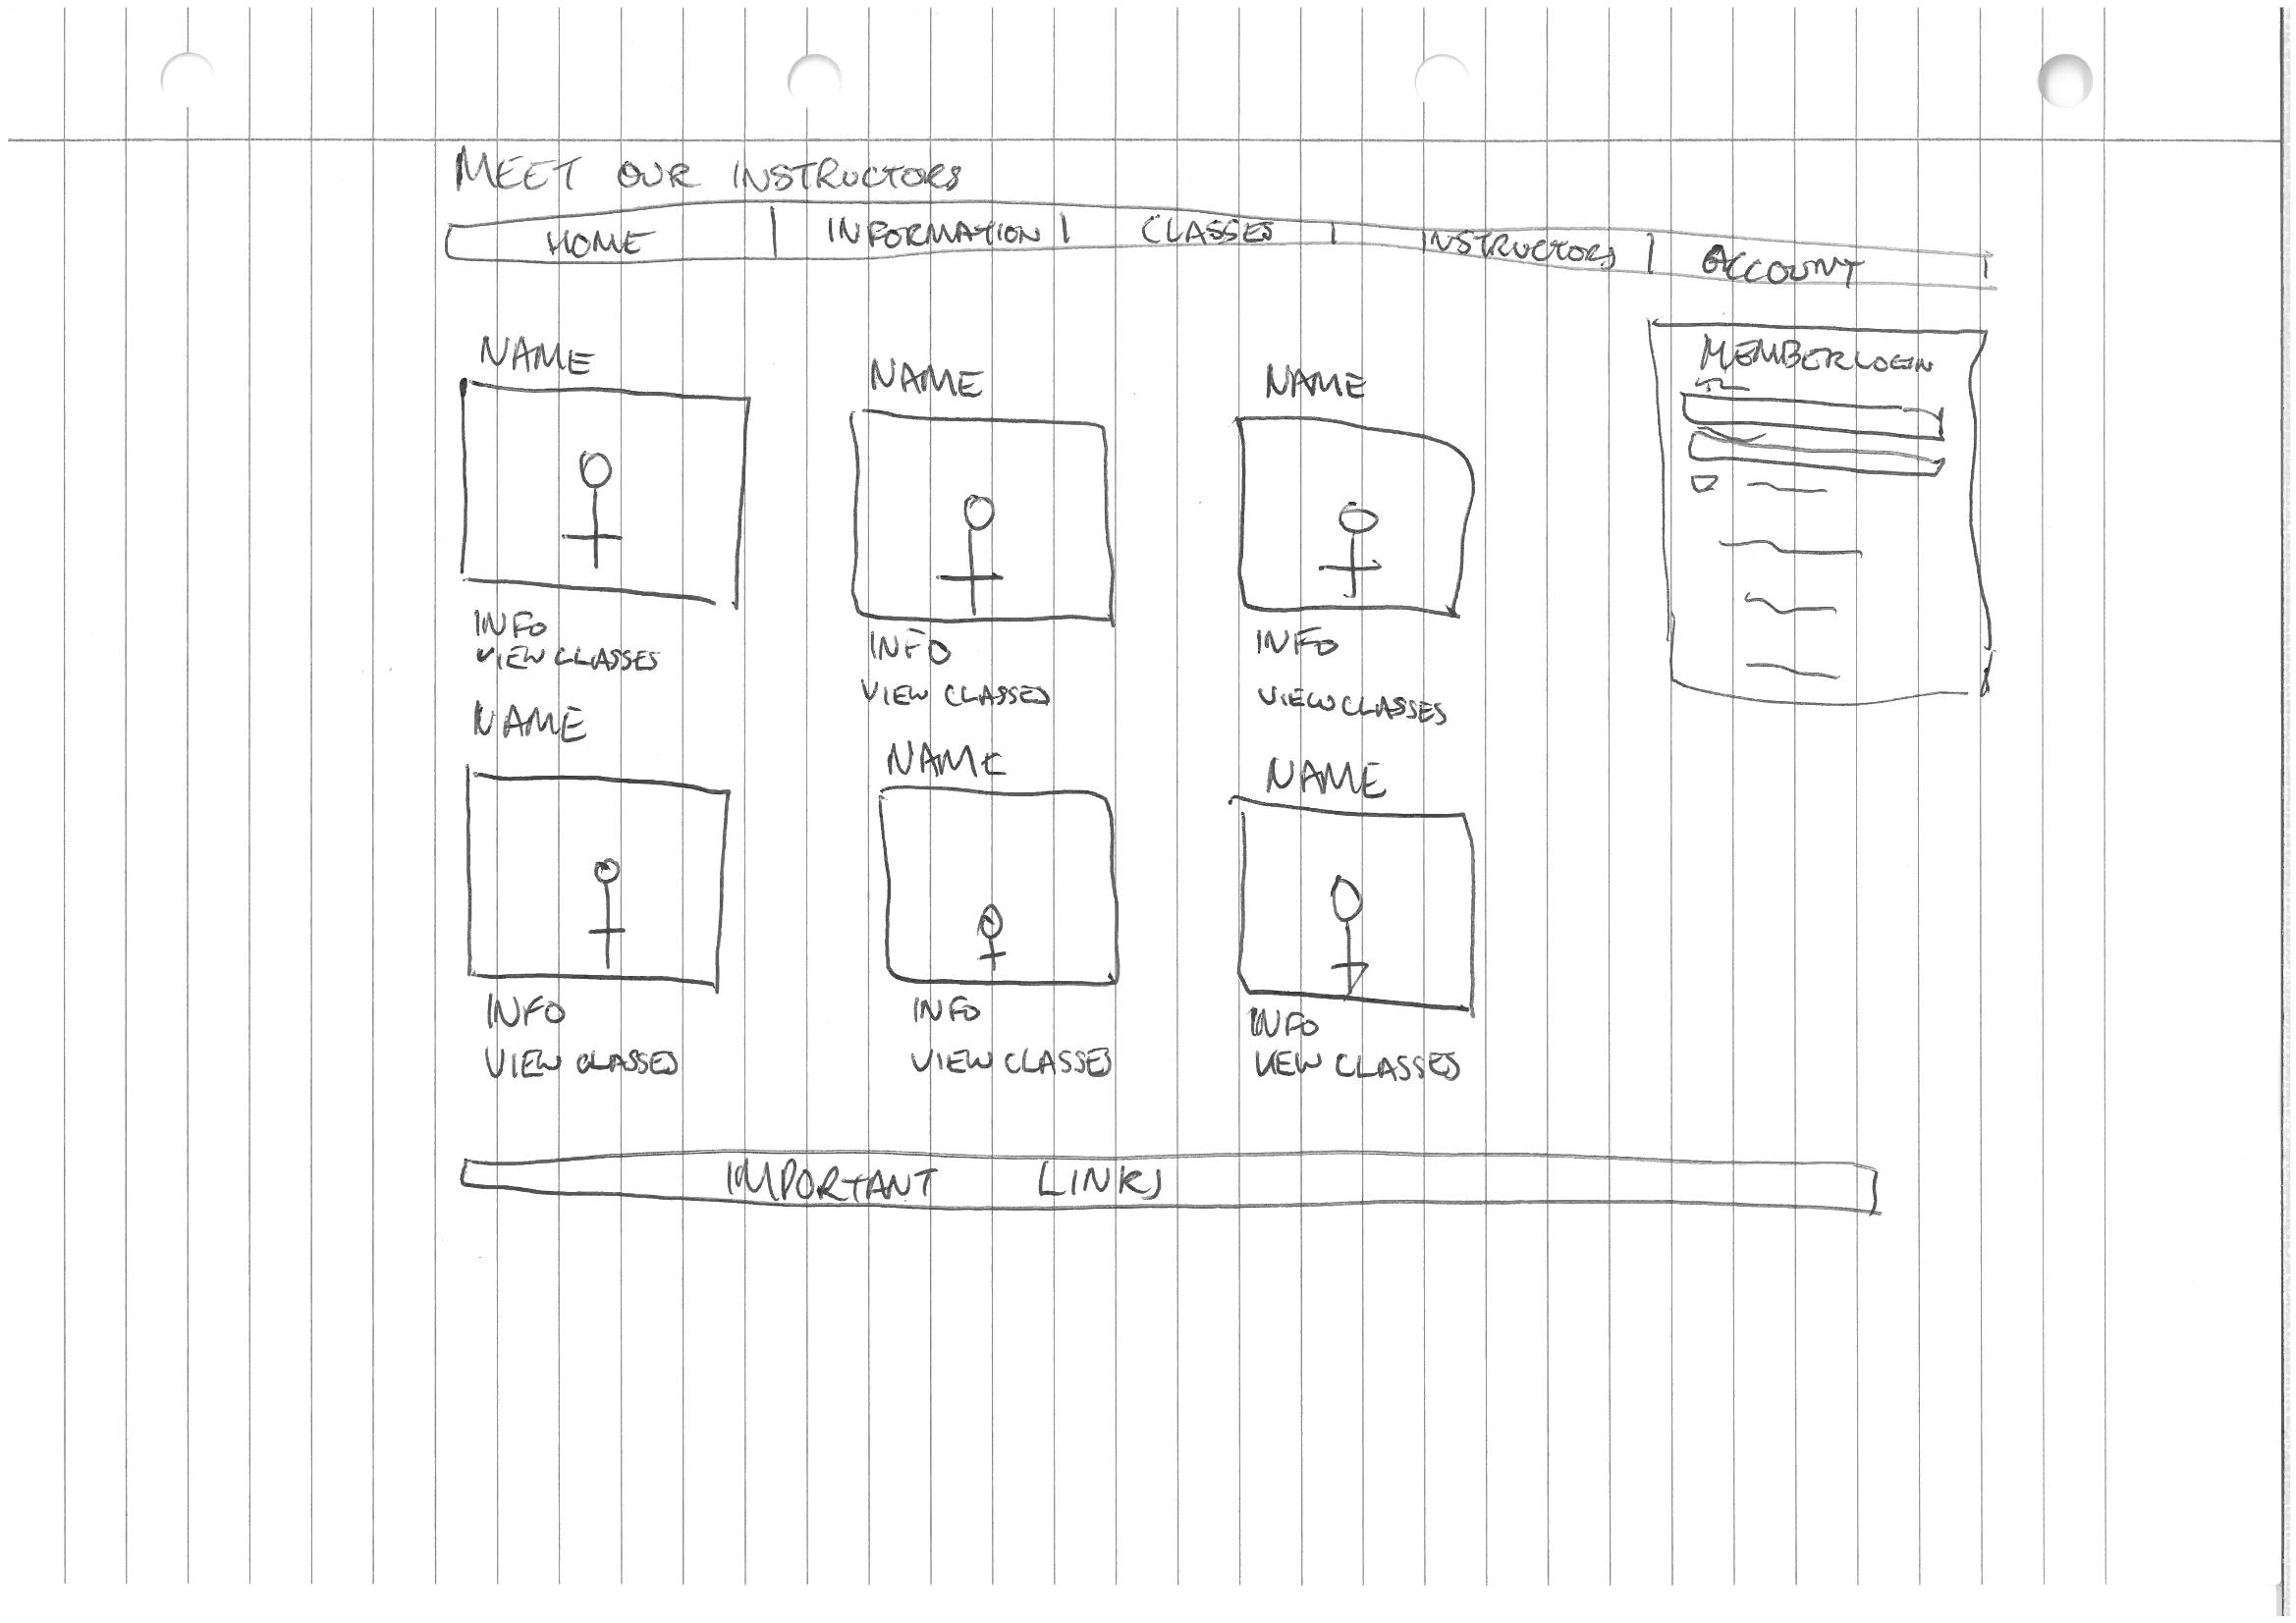
\includegraphics[scale=0.7]{images/instructorpage}
 	\caption{Instructors Listing Page}
	\end{figure}
	This page will be identical to the Classes page, allowing users to find more detail about instructors, and view the classes each instructors runs.
	\newpage
	

			\begin{figure}[ht!]
	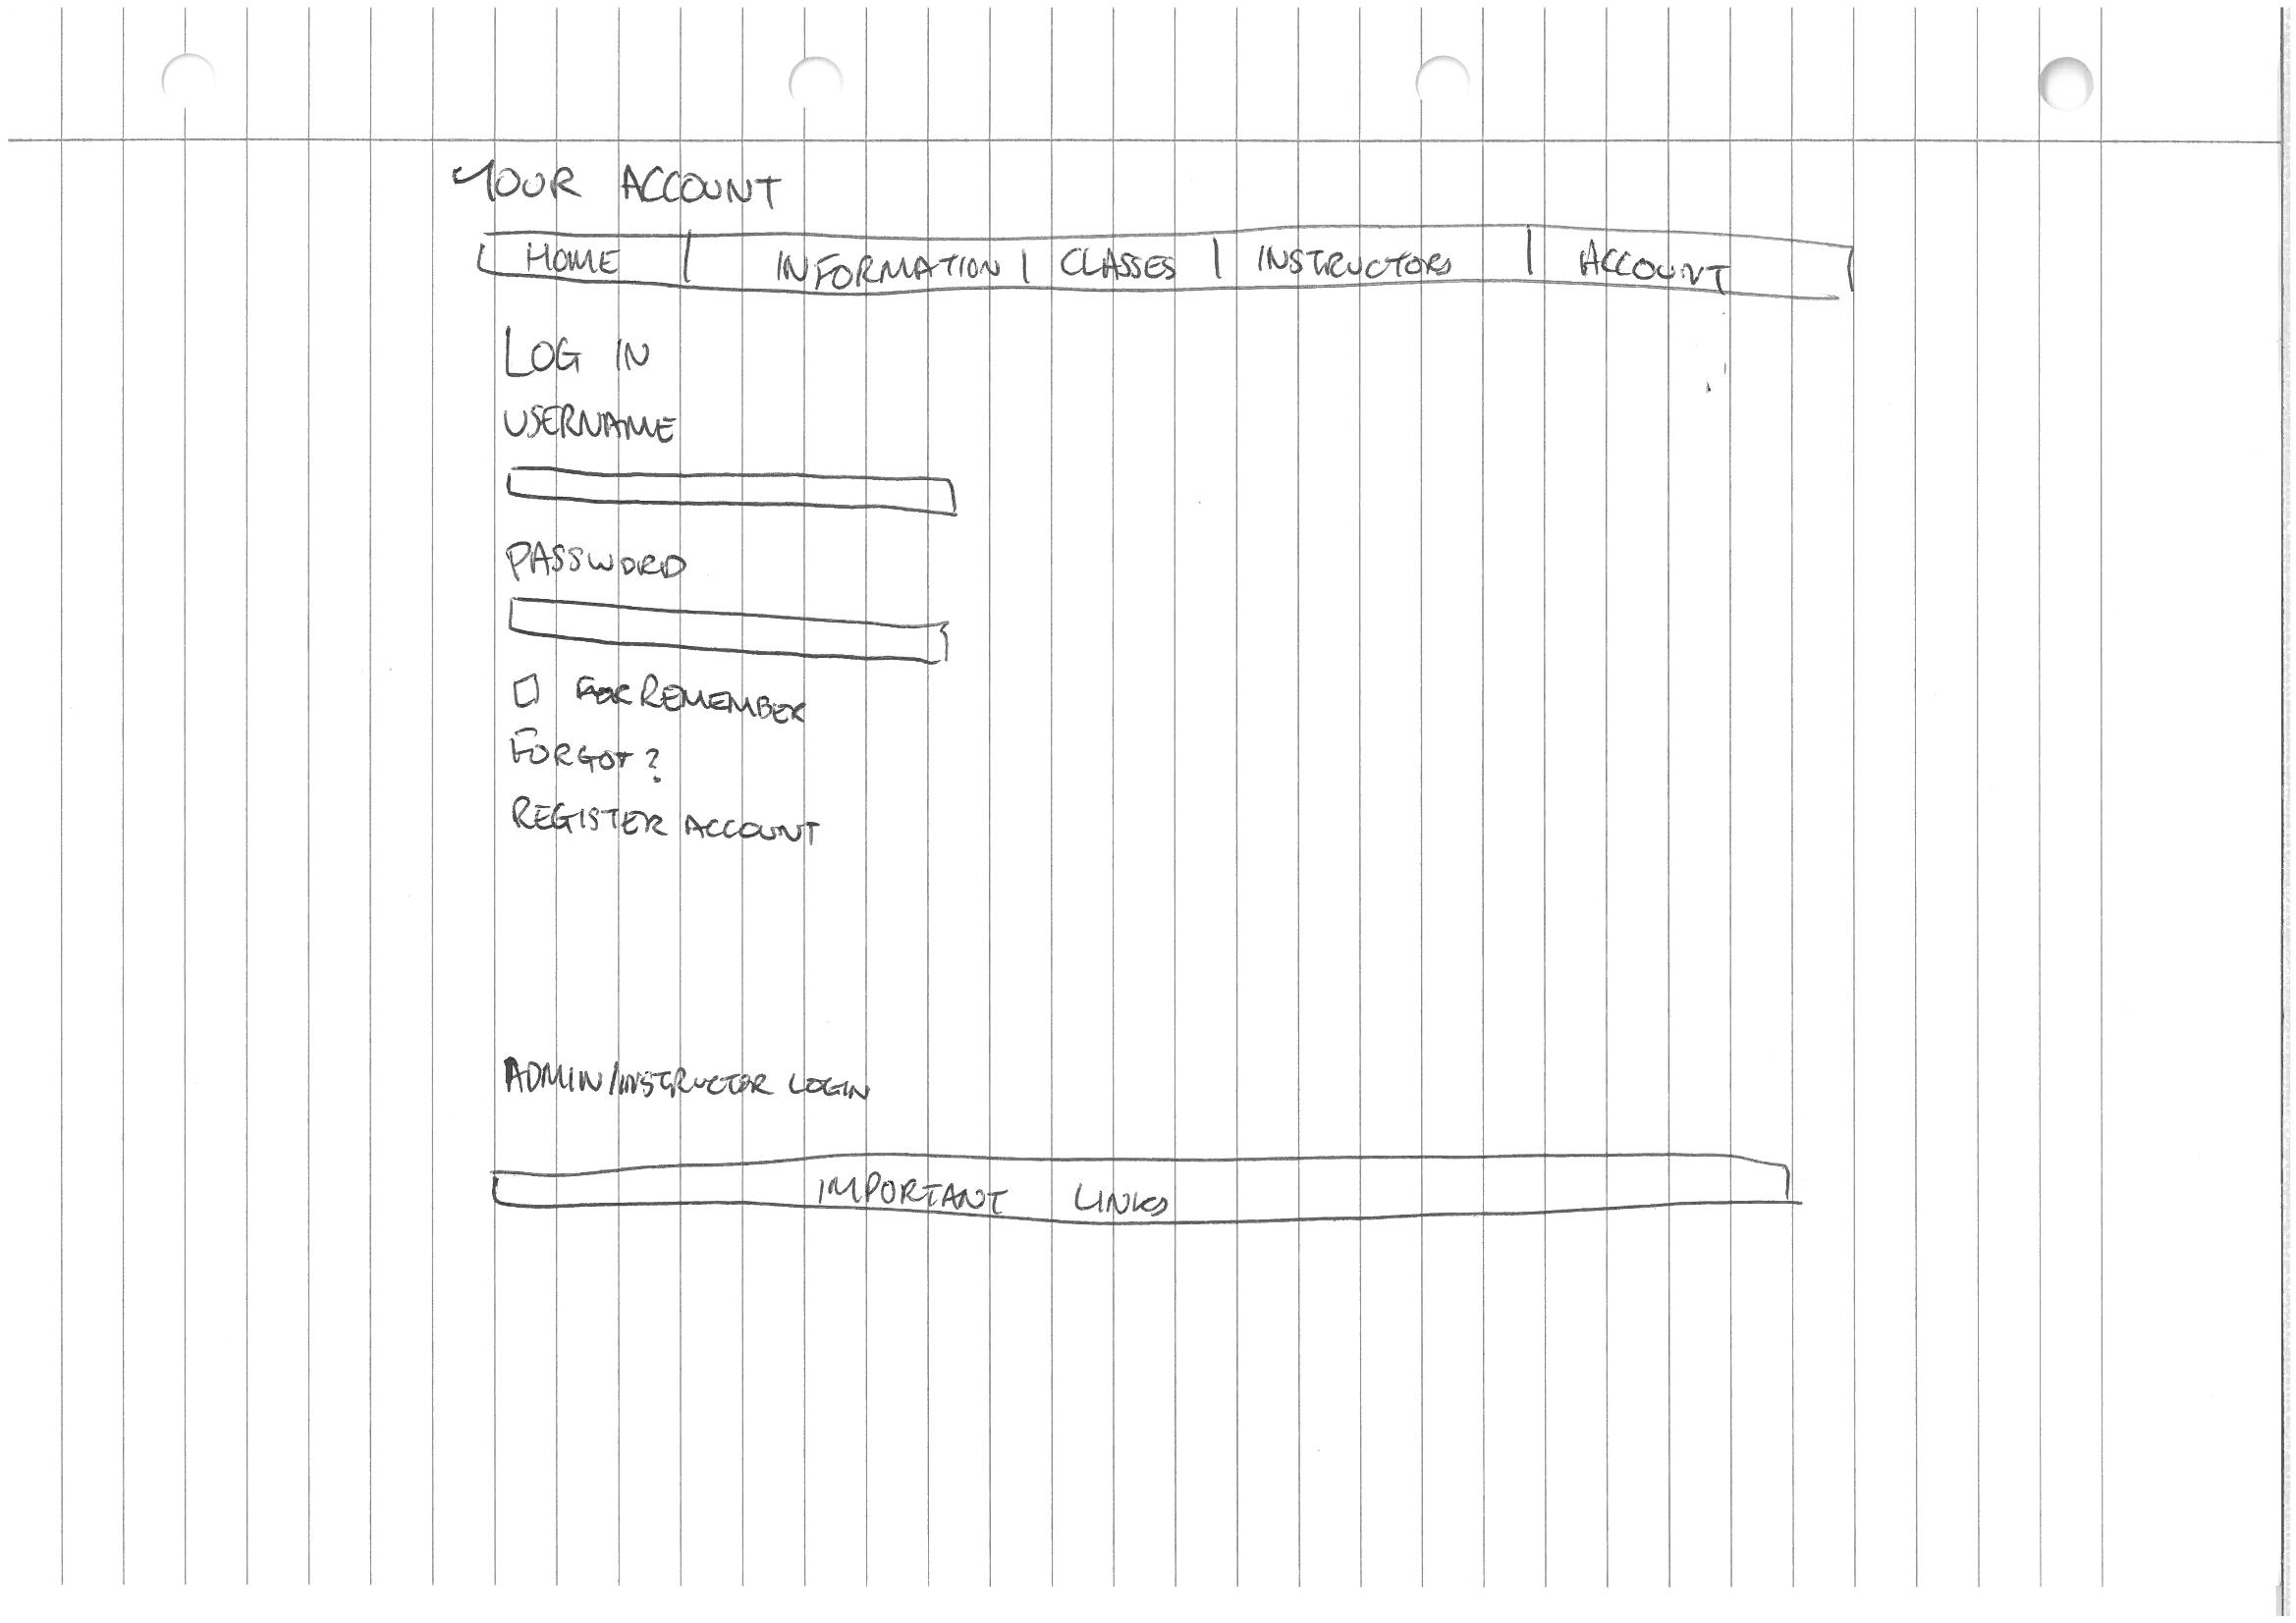
\includegraphics[scale=0.7]{images/loginpage}
 	\caption{Login Page}
	\end{figure}
	This page is an enlarged version of the side box used on previous pages. This is for users who fail to see the login box on other pages, in accordance to Schneiderman's 2nd and 7th rule.
	1: Aministrator and instructor login would, ideally, be automatically identified by the username inputted. However, for the assignment, I am going to supply to a separate login box to allow you to navigate to the admin/instructor account page.
	
	\newpage
			\begin{figure}[ht!]
	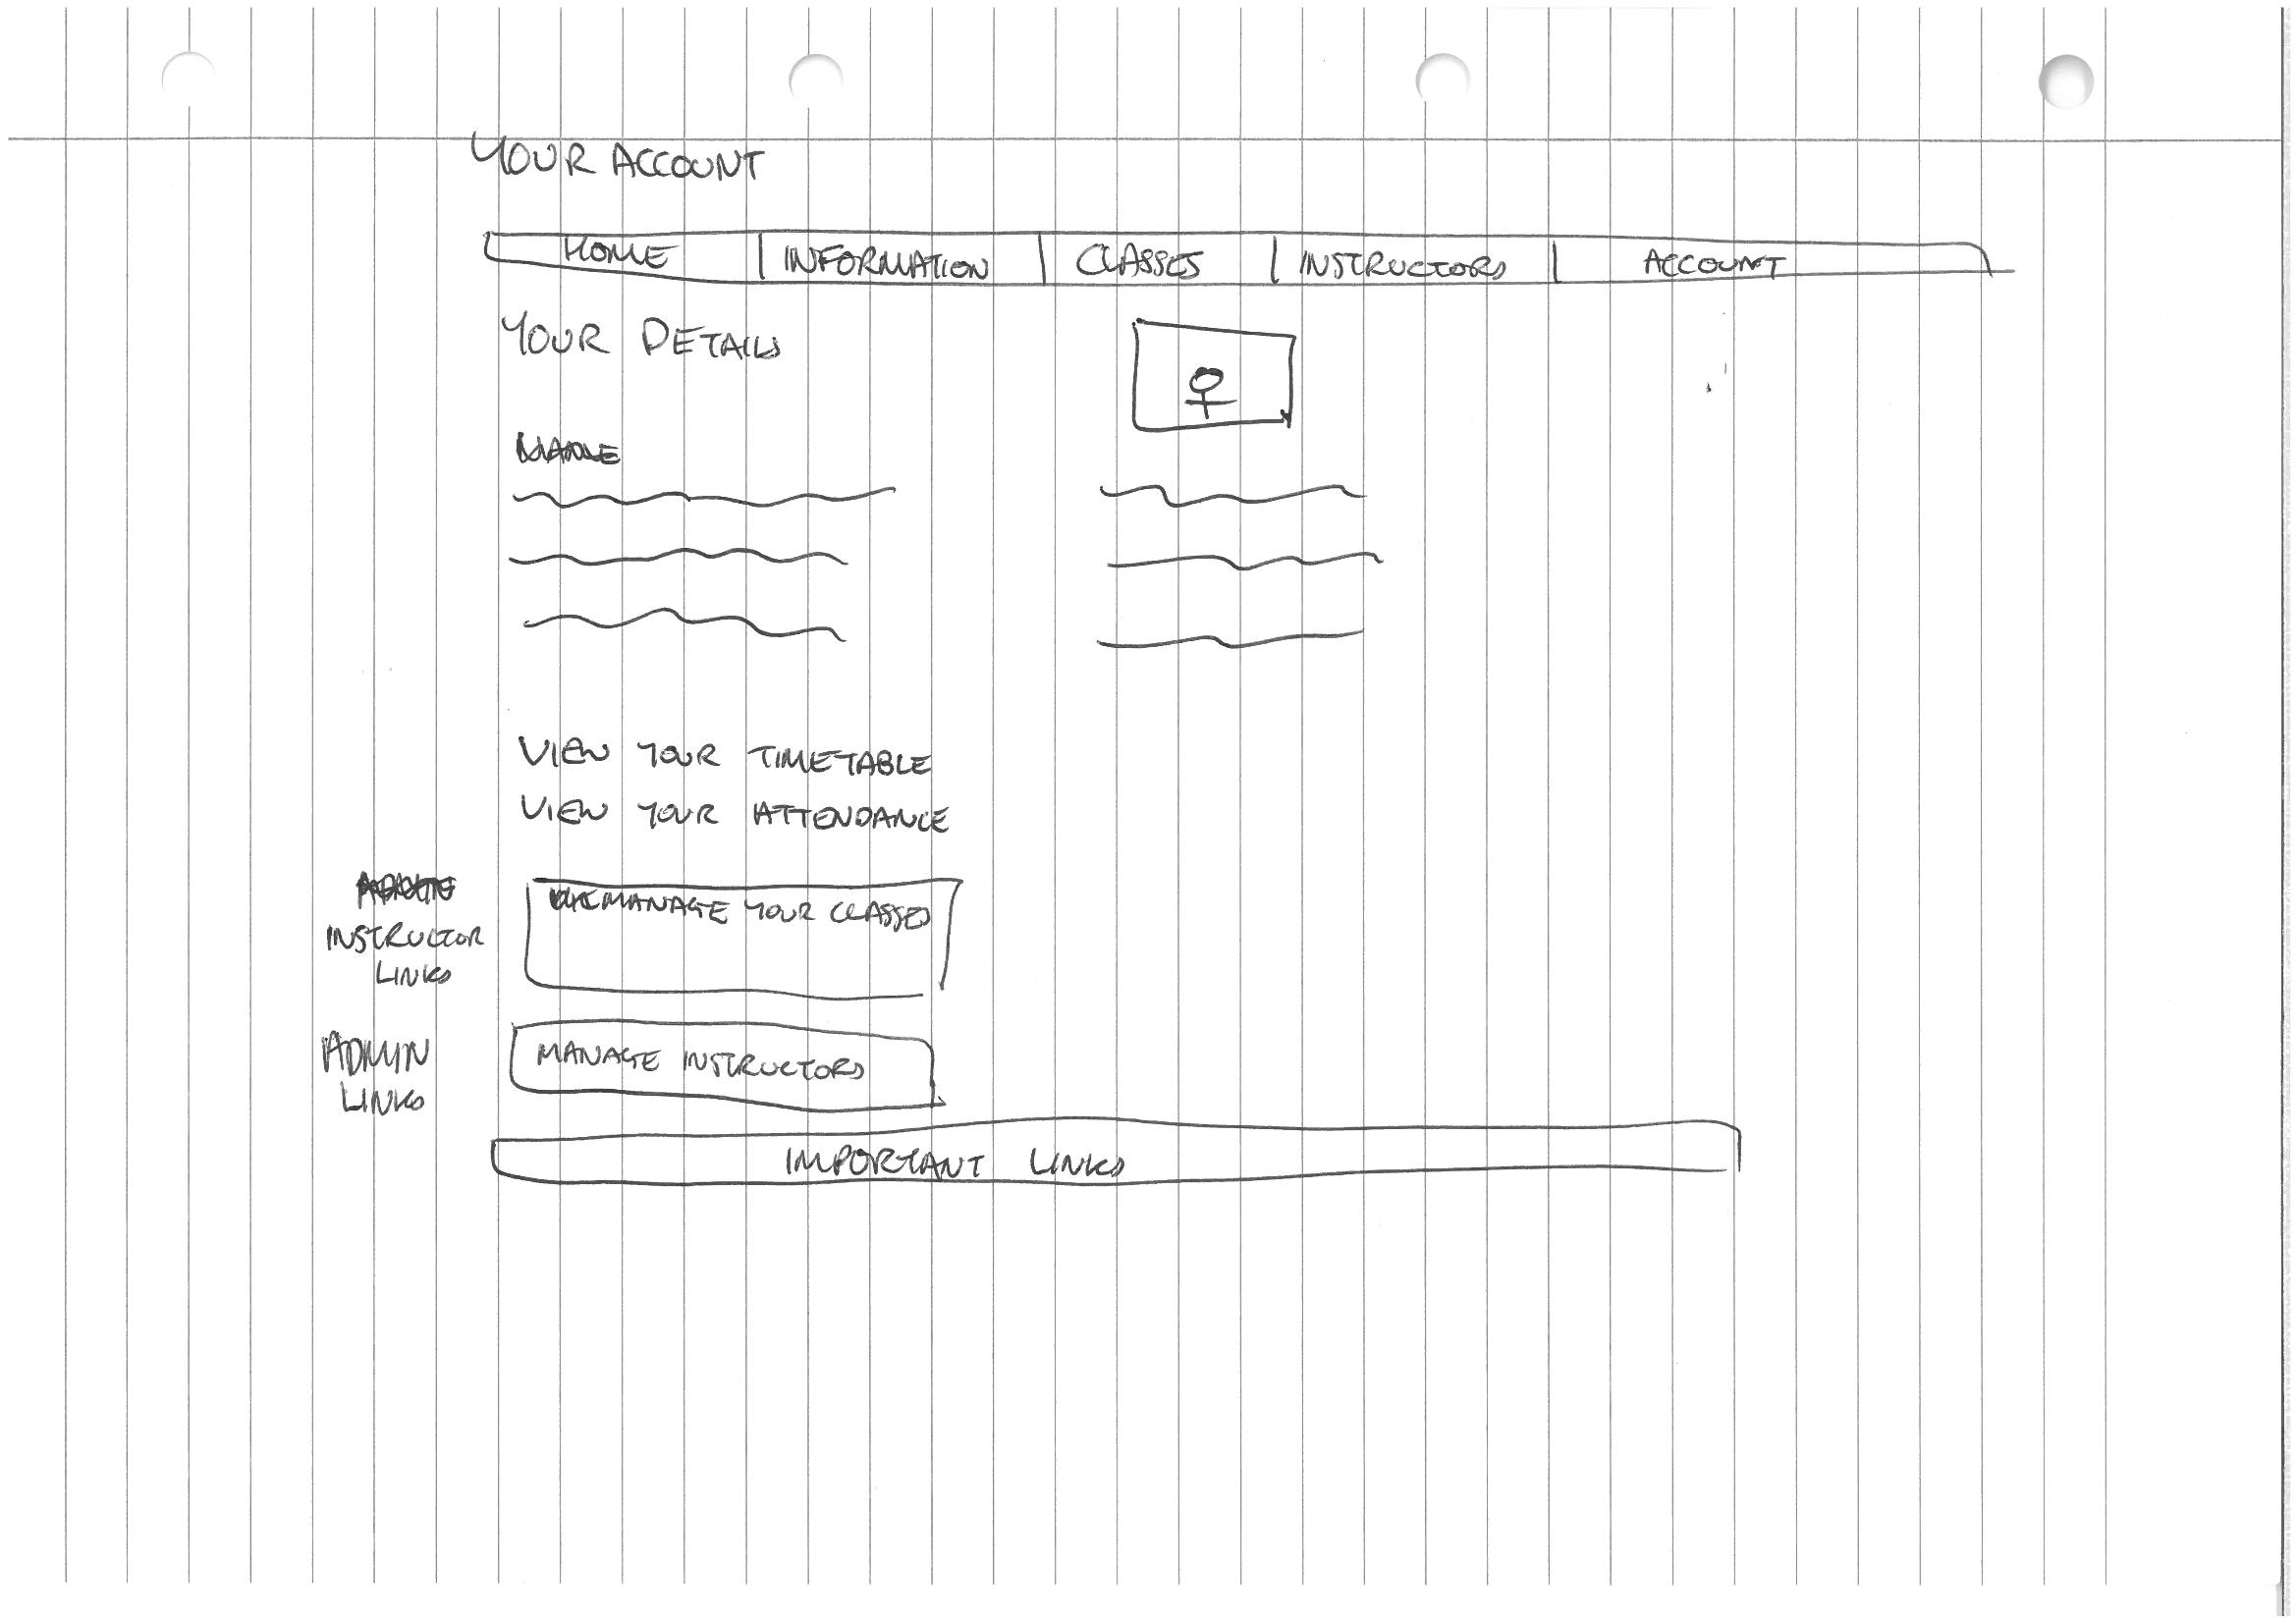
\includegraphics[scale=0.7]{images/loggedinaccpage}
 	\caption{Account Management Page}
	\end{figure}
	1: This text provides information supplied by the user upon registration. A picture is also displayed.
	
	2: Timetable and attendance links are provided to give the user control over their enrolment, according to Schneiderman's 6th and 7th rule.
	
	3: This link will only appear if the user is an instructor. This will allow them to manage their classes.
	
	4: This link and the previous link will appear if the user is an administrator. This will allow them to manage their instructors.

\section{Prototype Link}
My prototype link:

\url{users.aber.ac.uk/mta2/cs22310}
\newline \newline
All images on the site are royalty-free from this site:

\url{http://pixabay.com/en/}



	\section{Evaluation of Prototype}
	\subsection{Shneiderman's 8 Golden Rules}
	\subsubsection{1. Strive for Consistency}
	To meet this goal, I ensured a consistent yellow and black colour scheme throughout, to make sure the user knew he/she was still on the site. This also provides overall theme, making my site more identifiable. I also ensured links and buttons were consistent throughout, to ensure the user knew what sort of button would do what. The unique buttons tended to be links, whereas the more generic buttons were to login and text links were kept familiar.
	\subsubsection{2. Cater to Universal Usability}
	To do this, I ensured text was always easily visible using a nice and user-friendly colour scheme and font. The font size is kept consistent throughout the site to prevent strain on eyes with small text. If a user needed accessbility assistance on any page, an Accessbility section is displayed on the right providing three font choices and a high contrast mode. 
	
	\subsubsection{3. Offer Informative Feedback}
	To allow a user to know what button they are hovering over in the navigation bars, the background changes to yellow, and the text changes to black. This ensures the user knows exactly what they will click before they click. The text colour changes also ensures the user can still read the text. The user is then also told what page they are on by keeping the relevant navigation tab highlighted. For all other links/buttons, a cursor shape change is provided to let them know they can click on the link/button. 
	
	\subsubsection{4. Design Dialogs to Yield Closure}
	For this assignment, there was not much scope to achieve or fail this rule. The only way I can think of where this rule becomes relevant is where I have ordered the navigation bar and page content in order of relevancy to the most general user. For example, the navigation bar has the most relevant links towards the left, closer to the sweet spot; on the classes page, information about each class is shown first, then the link if the user has decided to enrol. 
	
	\subsubsection{5. Prevent Errors}
	By implementing HTML5's form validations, I have a lot of scope to prevent the few errors that can occur on this assignment. When registering a new account, I require all fields to be filled to ensure a user can not create an account with them. For entering an e-mail (as required by the spec), the e-mail validation input field is used to ensure a valid e-mail is inputted. Other input types are provided such as tel to ensure a phone number is entered, password to hide the password field from prying eyes. I would ideally like to implement an address finder that, based on the postcode, would find the correct address. I created two password entry fields, which, with JavaScript, would ensure a user enters the correct password. When entering a date range, the date input field is used to ensure the administrator can not enter wrong data into the date fields. This prevents errors from occuring and being overlooked which would cause confusing data to appear on the site.
	
	\subsubsection{6. Permit Easy Reversal of Actions}
	Again, I don't feel there was much scope to achieve or fail this rule. One way I can think of achieving this rule is having the ability to easily cancel enrolment on a class. A user can enrol on a class from the classes page, and then navigate to their account page to cancel it straight away. There is no fuss concerning this. Another example is when an administrator adds a new class or instructor. This can easily be reversed on the same page by clicking the remove class or remove instructor button. Edit class buttons have also been added to allow an administrator edit the time or an instructor edit the information of a class.
	
	\subsubsection{7. Support Internal Locus of Control}
	To allow the user feel in control, I have the user interface very simple. There are no confusing links or buttons that will take the user to an unexpected location on the site. If the user selects on the classes link, they are taken there; if the user logs in, they are logged in. By having simple navigation and relevant names on each link, the user knows what they are doing every step of the way, and never feels a loss of control.
	
	\subsubsection{8. Reduce Short-term Memory Load}
	To meet this rule, only relevant information for each page is displayed, with no irrelevant information shown. This reduces memory-load on the user by not forcing extra, unwanted information on them. For example, on the classes page, information is brief and to the point, with important links easily found. The pages are separated in a way that categorises information to support this. Pictures are also shown throughout to remind the user what type of content they are looking at. 
	
		\subsection{Personal Evaluation}
	Overall, I feel my site provides all the functionality needey as required by the project specification. I feel my site looks user-friendly and professional and is easy to navigate around, providing a nice user experience. A massive downfall of the site, however, is the user experience on mobile. I was not able to create as nice an experience for mobile users as I would have hoped, partly due to not realising Bootstrap was an option. Creating a responsive web design was very difficult, and I could not complete it successfully. I did, however, ensure that content was viewable on mobile, thus creating a usable website for mobile users. If I had more time to re-do this project, I would use bootstrap to ensure a user-friendly experience on all devices, or I would research further into creating a more responsive interface.

	%%\begin{landscape}

		%%\section{Bar}
			%%\input{far/foo.tex}

	%%\end{landscape}


\end{document}